\chapter{Automatisation du processus d'investigation}
\label{Automatisation du processus d'investigation}
\thispagestyle{fancy}
Lorsqu'une error name (partie \ref{Introduction:Expression du besoin:Hiérarchisation des erreurs}) durant le Filtering test, de nombreuses données du robot sont enregistrées dans un fichier journal (que l'on retrouve plus souvent sous le terme anglais de fichier "log".) Une analyse poussée des données contenues dans ce fichier nous permet de déterminer la root cause liée à l'error name (partie \ref{Introduction:Expression du besoin:Hiérarchisation des erreurs}). Afin d'automatiser ce processus d'analyse, on s'appuie sur l'utilisation d'algorithmes d'apprentissage automatique. 

\section{Architecture High Level du système proposé}
\label{Automatisation du processus d'investigation: Achitecture High Level du système proposé}
L'architecture haut niveau de la solution que l'on propose est composée de deux couches: une couche "root cause" et une couche "error name".
\begin{description}
	\item [Couche root cause] La couche root cause permet de détecter une root cause en analysant le fichier log.
	\item [couche error name] La couche error name est constituée d'un ensemble de couches error name, de telle manière que lorsqu'un fichier historique est mis en entrée du système, la couche error name active l'ensemble des couches root cause qu'elle contient. Ainsi, une analyse de chaque root cause sera effectué sur le fichier.
\end{description} 

Un schéma synoptique illustrant le fonctionnement systémique de notre architecture High Level est proposé figure \ref{fig:Schéma synoptique haut niveau de la solution proposée: couche root cause} et \ref{fig:Schéma synoptique haut niveau de la solution proposée: couche error name}.

\begin{figure}[h]
	\centering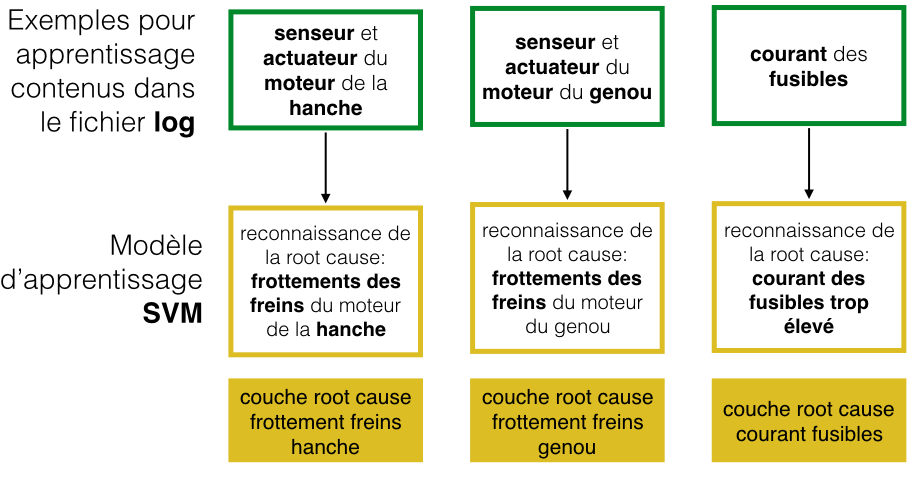
\includegraphics[height=7cm]{images/synoptique_root.png}
	\caption{Schéma synoptique haut niveau de la solution proposée}
	\label{fig:Schéma synoptique haut niveau de la solution proposée: couche root cause}
\end{figure}

\begin{figure}[h]
	\centering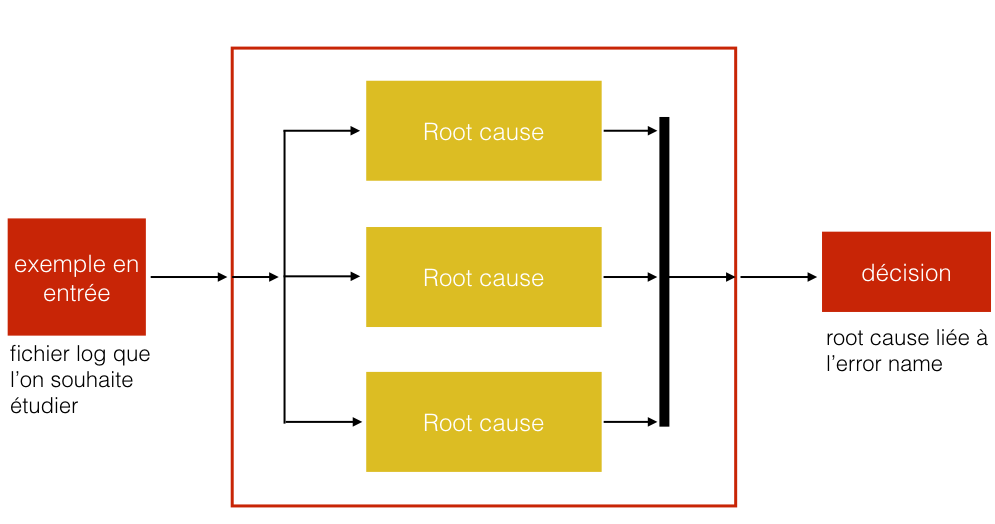
\includegraphics[height=7cm]{images/synoptique_error.png}
	\caption{Schéma synoptique haut niveau de la solution proposée}
	\label{fig:Schéma synoptique haut niveau de la solution proposée: couche error name}
\end{figure}

\subsubsection{Les exemples pour apprentissage et exemple à analyser}
\label{Automatisation du processus d'investigation: Achitecture High Level du système proposé: Les exemples d'apprentissage}

\subsubsection{Le modèle d'apprentissage}
\label{Automatisation du processus d'investigation: Achitecture High Level du système proposé: Le modèle d'apprentissage}

\subsubsection{La décision}
\label{Automatisation du processus d'investigation: Achitecture High Level du système proposé: La décision}



\section{Solutions techniques testées}
\label{Automatisation du processus d'investigation: Solutions techniques testées}




\section{Solution technique proposée}
\label{Automatisation du processus d'investigation: Solution technique proposée}

